 \begin{center}
\textbf{Lesson 2.11: Triangle Inequality Theorem}
\end{center}

%\vspace*{1ex}

\textbf{Triangle Inequality Theorem:} The sum of the lengths of any two sides of a triangle is greater than the length of the third side.

\begin{center}
\begin{minipage}[c]{0.48\textwidth}
\begin{flushright}
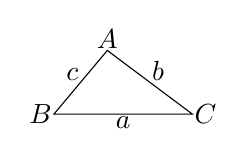
\begin{tikzpicture}%[remember picture, overlay] 

\def\len1{5em}
\def\leninnersep{2ex}

\draw (0,0) coordinate (b)  -- (50:0.6*\len1) coordinate (a) node[midway, anchor=south east, inner sep=0.07*\leninnersep, rotate=0] (c-mid) {$ c$} -- (0:\len1) coordinate (c) node[midway, anchor=south west, inner sep=0.07*\leninnersep, rotate=0] (b-mid) {$ b$} -- cycle node[midway, anchor=north, inner sep=0.1*\leninnersep, rotate=0] (a-mid) {$ a$}; 

\node[anchor=south, inner sep=0.07*\leninnersep, rotate=0] (a-label) at (a) {$ A$};

\node[anchor=east, inner sep=0.07*\leninnersep, rotate=0] (b-label) at (b) {$ B$};

\node[anchor=west, inner sep=0.07*\leninnersep, rotate=0] (c-label) at (c) {$ C$}; 

\end{tikzpicture} 
\hspace*{1em}
\end{flushright}
\end{minipage}
\begin{minipage}[c]{0.48\textwidth}
$ a + b > c $\\
$ b + c > a $\\
$ a + c > b $\\
\end{minipage}
\end{center}
